\documentclass[11pt]{article}

\usepackage[margin=0.6in]{geometry}
\usepackage[T1]{fontenc}
\usepackage[utf8]{inputenc}
\usepackage{lmodern}
\usepackage{array}
\usepackage{booktabs}
\usepackage{longtable}
\usepackage{tabularx}
\usepackage{caption}
\usepackage{float}
\usepackage{hyperref}
\usepackage{parskip}
\usepackage{ragged2e}
\usepackage{setspace}
\usepackage{enumitem}
\usepackage{needspace}
\usepackage[table]{xcolor}
\usepackage{tikz}
\usetikzlibrary{arrows.meta,positioning,fit}
\usepackage[natbibapa]{apacite}

\definecolor{PrimaryRed}{HTML}{8B1E1E}
\definecolor{DeepNavy}{HTML}{15324A}
\definecolor{MidTeal}{HTML}{287D7A}
\definecolor{SoftBlue}{HTML}{DDEEFF}
\definecolor{SoftGreen}{HTML}{E4F1E8}
\definecolor{SoftGold}{HTML}{F8EDC7}
\definecolor{SoftRose}{HTML}{F5E2E7}
\definecolor{SoftGray}{HTML}{F4F4F4}

\hypersetup{
  colorlinks=true,
  linkcolor=DeepNavy,
  urlcolor=DeepNavy,
  citecolor=DeepNavy,
  pdftitle={Communication That Travels With the Student},
  pdfauthor={Piter Zacari Garcia Bautista},
  pdfsubject={EDE 448 Module 3 Communication Support Plan},
  pdfkeywords={AAC, neurodivergence, CLD, bilingual communication, health-aware communication, nonspeaking students, Puzzle Plan, EQUITAS}
}
\setlength{\parindent}{0pt}
\setstretch{1.05}
\setlist[itemize]{leftmargin=0.23in,itemsep=0.02in,topsep=0.04in}
\captionsetup{font=small,labelfont=bf,labelsep=period}
\bibliographystyle{apacite}

\newcommand{\reviewsection}[1]{%
  \Needspace{4\baselineskip}
  \vspace{0.08in}\noindent{\normalsize\bfseries\color{PrimaryRed}#1}
  \par\vspace{0.025in}
}

\newcommand{\tableheaderthree}[3]{%
  \rowcolor{PrimaryRed}
  \color{white}\bfseries #1 &
  \color{white}\bfseries #2 &
  \color{white}\bfseries #3 \\
}

\newcommand{\tableheaderfour}[4]{%
  \rowcolor{PrimaryRed}
  \color{white}\bfseries #1 &
  \color{white}\bfseries #2 &
  \color{white}\bfseries #3 &
  \color{white}\bfseries #4 \\
}

\begin{document}

\hypersetup{pageanchor=false}
\begin{titlepage}
\newgeometry{margin=0.7in}
\thispagestyle{empty}

\begin{center}
{\large University of Rochester\\}
{\normalsize Warner School of Education\\[0.15in]}

{\color{PrimaryRed}\rule{\textwidth}{1.4pt}}\\[0.12in]
{\Huge\bfseries Communication That Travels\\[0.07in]
With the Student}\\[0.15in]
{\huge A Neurodiversity-Affirming,\\[0.06in]
Culturally and Health Responsive Support Plan}\\[0.12in]
{\Large AAC, Bilingual Access, Partner Practice, and Home--School Continuity}\\[0.14in]
{\large EDE 448 -- Module 3 Assignment}\\[0.10in]

\vfill

{\color{PrimaryRed}\rule{0.78\textwidth}{0.7pt}}\\[0.18in]

\colorbox{SoftBlue}{%
\parbox{0.88\textwidth}{%
\centering\small\vspace{0.02in}
\textbf{Communication Access Travels Across Languages, Bodies, Tools, Partners, Places, and Routines}\\[0.04in]
The plan centers three fictional composite neurodivergent learners and turns documented camp and teaching-placement strategies into concrete communication supports.
}%
}
\end{center}

\vfill

\begin{center}
\renewcommand{\arraystretch}{1.18}
\setlength{\tabcolsep}{4pt}
\begin{tabular}{>{\bfseries\RaggedLeft\arraybackslash}p{1.85in} >{\RaggedRight\arraybackslash}p{5.0in}}
Student & Piter Zacari Garcia Bautista \\
Assignment & Communication Support Plan \\
Course & EDE 448 -- Communication and Positive Behavioral Supports for Students with Autism and Other Complex Needs \\
Planning Context & Inclusive upper-elementary STEM and technology routines \\
Composite Learners & CLD bilingual communicator, speech/multimodal communicator, and chronically ill low-speaking communicator \\
Applied Experience & EDU486 Invisible Invaders camp and K--5 technology teaching placement \\
Interpretive Framework & Puzzle Plan, with EQUITAS at its heart \\
\end{tabular}
\end{center}

\vfill

\begin{center}
\begin{minipage}{0.92\textwidth}
\centering\itshape
The goal is reliable student authorship across people, places, languages, bodies, messages, and moments.\\
{\color{PrimaryRed}\rule{4.4in}{0.8pt}}
\end{minipage}
\end{center}

\vfill

\begin{center}
\begin{minipage}{0.95\textwidth}
\small
The three student profiles in this plan are fictional composites created for the assignment. Their neurodivergence, communication profiles, health needs, and support needs belong to the fictional characters. De-identified camp and teaching-placement records contribute documented instructional strategies, participation patterns, and examples of how access changed when adults adjusted the environment. The Puzzle Plan is my interdisciplinary framework for connecting lived experience, education, data, and research so that no single observation is treated as the whole person. EQUITAS is the equity-focused lens at the heart of that framework; it asks whose knowledge enters the plan, what context is missing, where bias may shape interpretation, and whether support expands dignity, agency, belonging, and access.
\end{minipage}
\end{center}

\restoregeometry
\end{titlepage}
\hypersetup{pageanchor=true}
\pagenumbering{arabic}

\reviewsection{Purpose and Student Design}

This plan supports three upper-elementary fictional composite students during inclusive STEM and technology routines and the home--school transition that follows them. Each student represents a puzzle piece in my Puzzle Plan and a puzzle piece in a learner's own life: Mateo represents neurodivergence, culture, and language; Eli represents neurodivergence and speech/multimodal access; and Luca represents neurodivergence, chronic illness, low speech, and speech-related trauma. The profiles are fictional. The support strategies are grounded in de-identified EDU486 camp evidence, K--5 teaching-placement evidence, and prior EDE448 work on access, agency, dignity, consent, and neurodiversity \citep{campEvidence2026,placementEvidence2026,garciabautista2026ptr,garciabautista2026module2journal}.

The assignment asks for a communication support plan for nonspeaking students. A three-student composite design lets me examine how nonspeaking, low-speaking, bilingual, health-affected, and speech-unreliable communication profiles require different supports while sharing the same core principle: a student's speech should not be the price of participation. The goal is reliable authorship. Each learner needs ways to initiate, refuse, repair, ask, comment, joke, explain, choose a role, protect sensory and body boundaries, influence the activity, and decide what information travels home.

\reviewsection{Three Student Profiles}

\small
\setlength{\tabcolsep}{4pt}
\begin{longtable}{>{\RaggedRight\arraybackslash}p{0.95in} >{\RaggedRight\arraybackslash}p{2.10in} >{\RaggedRight\arraybackslash}p{3.85in}}
\tableheaderthree{Student}{Communication Profile}{Primary Planning Response}
Mateo & Neurodivergent CLD Spanish--English communicator. He is nonspeaking in this fictional plan and communicates through bilingual AAC, typing, photographs, pointing, gesture, and familiar written words. & Keep Spanish and English visible; pair speech with modeled examples and first/next/last visuals; allow translanguaging; preload academic vocabulary such as \textit{code/código, build/construir, test/probar, change/cambiar, evidence/evidencia, help/ayuda}; never require English repetition after a clear Spanish message. \\
\rowcolor{SoftGray}
Eli & Neurodivergent student with a fictional speech production disability. Speech is possible in some moments but effortful and unreliable; AAC, gesture, facial expression, movement, objects, drawing, photographs, and occasional vocal approximations carry meaning. & Keep high-tech AAC, printed backup, gesture, objects, photographs, drawing, and partner-supported access available; connect vocabulary to tools, evidence, roles, choices, and authentic audiences; use observe-first, pass, movement/reset, and return routes. \\
Luca & Neurodivergent chronically ill low-speaking student with speech-related trauma. He is not mute; speech may be unavailable when tired, in pain, returning from absence, or under adult pressure. & Protect health-aware pacing, privacy, and re-entry; provide check-in choices such as \textit{ready, observe, later, break, pain, tired, private, no voice today}; allow asynchronous contribution; avoid public demands for explanation; treat low speech as communication-access information, not refusal. \\
\end{longtable}
\normalsize

Teaching-placement evidence directly informs Mateo's profile. In one documented technology lesson, a student interface appeared in Spanish during stepwise editing support. The interaction continued through visual demonstration, pointing, and short directions; the student completed the editing step and the group moved into successful production work during the same session \citep{placementEvidence2026}. EDU486 camp evidence informs Eli and Luca. Youth could identify current energy, self-select meaningful roles such as commentator, and participate through measuring, observing, writing, pointing, photographing, partnering, voting, passing, returning, and revising shared models \citep{campEvidence2026}. Those are communication routes, not extra accommodations.

\reviewsection{Documented Practice Becomes Planned Support}

The composite profiles allow real instructional evidence to improve practice while keeping diagnosis, health history, and disability details inside the fictional scenario. The strongest strategies become explicit supports that any member of the team can reproduce.

\small
\setlength{\tabcolsep}{4pt}
\begin{longtable}{>{\RaggedRight\arraybackslash}p{1.42in} >{\RaggedRight\arraybackslash}p{2.06in} >{\RaggedRight\arraybackslash}p{1.66in} >{\RaggedRight\arraybackslash}p{1.65in}}
\tableheaderfour{Documented Practice}{Instructional Meaning}{Student Fit}{Planned Safeguard}
Stepwise technology support & Visual demonstration and short directions preserved progress during interface complexity \citep{placementEvidence2026}. & Mateo & Screenshots, bilingual labels, one visible step, AAC/typing response, and interface-language checks. \\
\rowcolor{SoftGray}
Youth-selected role & A meaningful role opened a communication route and gave the learner social purpose \citep{campEvidence2026}. & Eli & Commentator, evidence finder, photographer, demonstrator, observer/returner, and other flexible roles. \\
Energy and health check & Current body state informed access while competence remained visible \citep{campEvidence2026}. & Luca & Tired/pain/private/no voice today options, lower-output participation, rest, and planned re-entry. \\
\rowcolor{SoftGray}
Model revision and advocacy & Student contributions changed shared products and decisions \citep{campEvidence2026}. & All three & Communication must alter pace, role, tool, question, material, record, or next instructional decision. \\
\end{longtable}
\normalsize

\reviewsection{Adult Partner Practice as Communication Access}

One camp-based pattern also needs to enter the plan: adult partner behavior can either invite communication or shut it down. In de-identified records and field reflection, rigid adult direction, premature suggestions, long teacher talk, visible frustration, correcting by taking over materials, and returning to students while dysregulated functioned as access barriers. I do not need to name an adult to use the pattern responsibly. EQUITAS requires me to ask how power, race, disability, health, language, and adult authority shape what students feel safe enough to communicate.

The teaching lesson is direct: students need adults who regulate themselves before regulating the activity. A communication plan cannot only train the student to produce clearer messages. It must train partners to ask before suggesting, protect student authorship, avoid undoing student work, notice fear and shutdown as data, and repair when adult behavior reduces safety. For Black, CLD, neurodivergent, chronically ill, or low-speaking students, adult escalation can carry extra threat because the student may not have equal social power or equal access to explanation.

\small
\setlength{\tabcolsep}{4pt}
\begin{longtable}{>{\RaggedRight\arraybackslash}p{1.70in} >{\RaggedRight\arraybackslash}p{2.45in} >{\RaggedRight\arraybackslash}p{2.55in}}
\tableheaderthree{Partner Risk}{Why It Matters}{Replacement Practice}
Premature suggestions & Students may replace their ideas with the adult's idea because the adult holds instructional power. & Ask: ``What are you trying to make?'' ``What do you want this to do?'' Offer suggestions only after the student asks or shows they are stuck. \\
\rowcolor{SoftGray}
Taking over or undoing work & Correction can erase student authorship and make risk-taking feel unsafe. & Use a no-touch/no-undo rule: ask permission, describe the concern, offer choices, and let the student decide what changes. \\
Long talk and rigid pacing & Students may look bored, tired, quiet, or noncompliant when the barrier is adult pacing. & Use brief prompts, wait time, visual choices, movement, material access, and check-ins. \\
\rowcolor{SoftGray}
Visible adult dysregulation & Students can shut down when adult affect signals conflict, pressure, or danger. & Step away from students, co-regulate with another adult, return with a calm repair, and document the partner barrier. \\
\end{longtable}
\normalsize

\reviewsection{A Multimodal, Bilingual, and Health-Aware System}

\citet{mirenda2015aids} describes AAC as a continuously updated combination of aided and unaided techniques. ASHA identifies AAC as appropriate across ages and support profiles \citep{ashaAAC}. \citet{schlosser2014aac} emphasize communication functions, partners, settings, maintenance, and generalization, while \citet{weng2016language} makes the learner's language, family, and community part of feature matching. These principles support a system that travels through the student's real day.

\renewcommand{\arraystretch}{1.18}
\setlength{\tabcolsep}{5pt}
\begin{tabularx}{\textwidth}{>{\RaggedRight\arraybackslash}p{1.48in} >{\RaggedRight\arraybackslash}X >{\RaggedRight\arraybackslash}X}
\tableheaderthree{Component}{Purpose}{Access Safeguard}
Primary AAC device & Core, personalized, academic, social, sensory, health, and repair language & Charged, positioned, and available through the full routine; never removed as punishment or as a test condition \\
\rowcolor{SoftGray}
Low-tech backup & Stable access during charging, hands-on materials, positioning changes, illness, fatigue, or student preference & Preserve important words and predictable locations from the primary system \\
Spanish--English vocabulary & Language choice, family continuity, identity, and academic access & Student and family help choose vocabulary and preferred labels in both languages \\
\rowcolor{SoftGray}
Health and body vocabulary & Pain, fatigue, privacy, absence, medication-related needs, and re-entry & Keep \textit{tired, pain, private, no voice today, slower, later, ready, break,} and \textit{return} easy to access \\
Gesture, expression, movement & Existing efficient communication & Partners notice, confirm, and respond without demanding device repetition \\
\rowcolor{SoftGray}
Objects, photos, drawing, typing & Concrete and visual routes for academic and social meaning & Use these routes for open communication, explanation, questions, disagreement, and repair \\
Shared visual sequence & Comprehension, predictability, transition support, and return after absence & Show first/next/last, optional routes, changes, and re-entry points \\
\rowcolor{SoftGray}
Repair vocabulary & Fast correction after misunderstanding & Keep \textit{wait, not that, show me, different, another way, you misunderstood, something else} visible \\
\end{tabularx}

\reviewsection{Communication Must Cover the Full Message Range}

All three systems support greeting, social connection, choosing, refusing, commenting, questioning, directing a partner, expressing pain or sensory boundaries, predicting, comparing, explaining, labeling, revising, disagreeing, joking, asking for help or more time, repairing misunderstandings, choosing or changing a peer role, teaching another person, and deciding what information travels home. \citet{peckhamhardin2015behavior} connect functional communication with meaningful outcomes. A message becomes dependable when the partner response shows the student that communication can influence the environment.

\begin{figure}[H]
\centering
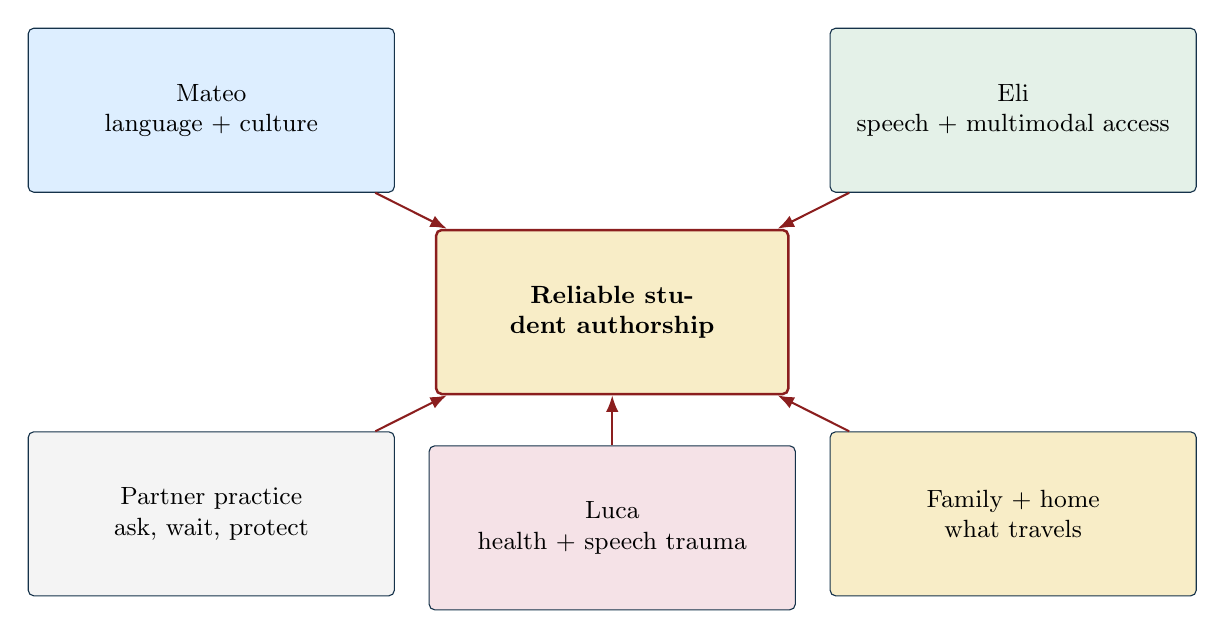
\begin{tikzpicture}[
  node distance=0.18in,
  piece/.style={draw=DeepNavy, rounded corners=2pt, text width=1.72in,
    minimum height=0.82in, align=center, font=\small, inner sep=4pt},
  centerpiece/.style={draw=PrimaryRed, line width=0.9pt, rounded corners=2pt, fill=SoftGold,
    text width=1.65in, minimum height=0.82in, align=center, font=\small\bfseries, inner sep=4pt},
  flow/.style={-{Latex[length=2.1mm]}, line width=0.75pt, draw=PrimaryRed}
]
\node[centerpiece] (center) {Reliable student authorship};
\node[piece, fill=SoftBlue, above left=0.18in and 0.20in of center] (mateo) {Mateo\\language + culture};
\node[piece, fill=SoftGreen, above right=0.18in and 0.20in of center] (eli) {Eli\\speech + multimodal access};
\node[piece, fill=SoftRose, below=0.25in of center] (luca) {Luca\\health + speech trauma};
\node[piece, fill=SoftGray, below left=0.18in and 0.20in of center] (partner) {Partner practice\\ask, wait, protect};
\node[piece, fill=SoftGold, below right=0.18in and 0.20in of center] (family) {Family + home\\what travels};
\draw[flow] (mateo) -- (center);
\draw[flow] (eli) -- (center);
\draw[flow] (luca) -- (center);
\draw[flow] (partner) -- (center);
\draw[flow] (family) -- (center);
\end{tikzpicture}
\caption{The three fictional learners show that AAC planning must connect language, speech access, health, partner behavior, and home continuity instead of treating communication as a device-only problem.}
\label{fig:puzzle-communication}
\end{figure}

\reviewsection{Communication Opportunity Matrix}

\citet{downing2015classroom} support embedding communication opportunities in ordinary classroom routines and peer interactions. The matrix gives all three students authentic communication work throughout the activity.

\small
\setlength{\tabcolsep}{4pt}
\begin{longtable}{>{\RaggedRight\arraybackslash}p{0.84in} >{\RaggedRight\arraybackslash}p{3.37in} >{\RaggedRight\arraybackslash}p{2.55in}}
\tableheaderthree{Routine}{Student Communication Routes}{Partner Action}
\endfirsthead
\tableheaderthree{Routine}{Student Communication Routes}{Partner Action}
\endhead
Arrival & Mateo chooses language and first task; Eli checks schedule or observes first; Luca selects ready, tired, private, no voice today, or later. & Review visible sequence, model vocabulary, protect wait time, and avoid demanding public explanation. \\
\rowcolor{SoftGray}
Technology setup & Mateo identifies interface language and requests a demonstration; Eli requests device position or access route; Luca chooses lower-output role or return point. & Keep systems within reach, demonstrate one step, and check whether fatigue or language changed access. \\
Observe & Students label, photograph, compare, point, reject material, choose tool, ask, pass, or direct attention. & Accept AAC, typing, gesture, photos, objects, drawing, bilingual language, and low speech as valid meaning. \\
\rowcolor{SoftGray}
Build/revise & Students explain or show a change, add or remove, label, disagree, direct a partner, or ask for clarification. & Ask before touching materials; do not undo work; offer choices only after learning the student's intent. \\
Group decision & Students vote, write in, point, pass, request time, identify an access barrier, or propose another option. & Make vote, write-in, pass, and return routes visible; record student influence on the decision. \\
\rowcolor{SoftGray}
Peer role & Students choose coder, director, recorder, translator by choice, commentator, evidence finder, photographer, demonstrator, materials lead, or observer/returner. & Let students combine, switch, redesign, or pause roles without losing belonging. \\
Reflection & Students use AAC, typed bilingual recap, photo, drawing, object, video/audio memo, or partner-supported summary. & Preserve student meaning before adult summary and let the student revise or restrict what is shared. \\
\rowcolor{SoftGray}
Home bridge & Students choose a message, artifact, question, vocabulary need, contribution, barrier, health/access note, or privacy option. & Student reviews, revises, restricts, or declines outgoing information; family can respond in any accessible language or mode. \\
\end{longtable}
\normalsize

\reviewsection{Communication Partner Plan}

Adults and peers will keep each communication system within reach, model language on a partner display, ask one question at a time, protect processing time, notice all reliable modes, confirm unclear meaning, ask before helping, return control after assistance, address the student directly, honor language choice, and respond when the student communicates refusal, correction, disagreement, pain, sensory boundaries, or a request for another route.

For Mateo, partners treat Spanish and English as usable communication resources and keep bilingual repair vocabulary visible. For Eli, partners watch for gesture, body movement, objects, photographs, drawing, and AAC as part of the same message system. For Luca, partners treat fatigue, absence, quietness, and speech avoidance as access data and keep health/privacy vocabulary available. When meaning is unclear, a partner can describe the observed action and offer a repair route: ``I saw you move the sample away. Are you saying \textit{stop}, \textit{different tool}, \textit{need space}, \textit{otra manera}, or something else?'' The student can confirm through any reliable mode.

\reviewsection{Flexible Peer Roles and Participation Routes}

Peers learn four actions: \textbf{invite, wait, ask, and respect}. They invite a real role, wait for the student's response, ask before helping or speaking for someone, and respect a role change, different language, quieter route, pass, health break, or later return. Possible roles include starter/modeler, coder, evidence finder, recorder/mapper, connector/questioner, reviser/debugger, materials/access lead, commentator, photographer, presenter/demonstrator, translator when voluntarily chosen, and observer/returner. Every role carries meaningful intellectual work and can change during the activity.

\reviewsection{Student-Centered Bilingual Home--School Record}

The supplied \textit{Daily Communication Logs} packet provides many school--home formats \citep{dailylogs2009}. This plan uses a record that carries student meaning, language, context, health access, and family knowledge across settings.

\setlength{\tabcolsep}{5pt}
\begin{tabularx}{\textwidth}{>{\bfseries\RaggedRight\arraybackslash}p{2.75in} >{\RaggedRight\arraybackslash}X}
\rowcolor{PrimaryRed}
\color{white}\bfseries Field & \color{white}\bfseries Student-Centered Entry \\
Student-authored or student-approved message to home & \\
\rowcolor{SoftGray}
Language(s), communication mode(s), and health/access status & \\
Activity and environmental conditions & \\
\rowcolor{SoftGray}
What the student chose, refused, asked, commented, taught, repaired, or protected & \\
Support that increased access & \\
\rowcolor{SoftGray}
Barrier or condition to change tomorrow & \\
Question, unfinished idea, or re-entry need after absence & \\
\rowcolor{SoftGray}
New vocabulary needed in Spanish, English, health access, sensory access, or repair & \\
Family message, vocabulary, context, or question for school & \\
\rowcolor{SoftGray}
Student reviewed outgoing message & Approved / changed / restricted / chose not to send \\
\end{tabularx}

Family knowledge can change vocabulary, materials, sensory planning, examples, routines, health-aware pacing, and goals. Families can respond through Spanish, English, another language, photographs, audio, written notes, or another accessible form. The student helps decide what information travels between settings.

\reviewsection{Implementation Sequence}

\small
\setlength{\tabcolsep}{4pt}
\begin{longtable}{>{\RaggedRight\arraybackslash}p{0.95in} >{\RaggedRight\arraybackslash}p{3.35in} >{\RaggedRight\arraybackslash}p{2.45in}}
\tableheaderthree{Time}{Team Action}{Student Control and Evidence}
Before Day 1 & Meet with student, family, SLP, and teacher; confirm modes, languages, access, interests, vocabulary, privacy, sensory needs, health-aware pacing, re-entry routines, and preferred roles; prepare primary and backup systems. & Student and family identify vocabulary, language preferences, supports, health/privacy boundaries, interests, and information-sharing choices. \\
\rowcolor{SoftGray}
Days 1--2 & Establish predictable system placement, visual sequence, bilingual vocabulary, health and sensory routes, partner wait/modeling practices, and adult regulation safeguards. & Record which routes each student chooses and where communication becomes easier or harder. \\
Days 3--5 & Embed communication in observation, technology use, building, peer roles, group decisions, reflection, dismissal, and return after absence. & Track initiations, questions, comments, refusals, repairs, role changes, language choices, health/access messages, and messages that change the activity. \\
\rowcolor{SoftGray}
Day 5 review & Student, family, teacher, SLP, and staff conduct a keep/change/add/remove review. & Student and family revise vocabulary, routes, sensory supports, partner practices, health pacing, or home--school fields. \\
Days 6--10 & Generalize across partners, materials, locations, academic tasks, energy levels, and language demands. & Check whether meaning survives changes in partner, language demand, tool, body state, and setting. \\
\rowcolor{SoftGray}
Day 10 decision & Team conducts a joint review of access, message range, agency, partner behavior, and implementation. & Student and family participate in deciding the next version of the plan. \\
\end{longtable}
\normalsize

\citet{norrie2021context} show that AAC adoption depends on training, technical support, staffing, coordination, and daily context. Responsibility therefore sits across the team: the teacher prepares communication opportunities, the SLP supports access and vocabulary organization, classroom staff maintain high- and low-tech availability, the family contributes language, health, and context, and the student directs priorities through ongoing feedback.

\reviewsection{Data, Review, and Success}

The team collects enough evidence to change support while keeping the student's communication at the center. The review focuses on availability, message range, initiation, repair, partner response, language access, sensory and health access, and whether communication produces a meaningful consequence.

\small
\setlength{\tabcolsep}{4pt}
\begin{longtable}{>{\RaggedRight\arraybackslash}p{1.45in} >{\RaggedRight\arraybackslash}p{2.55in} >{\RaggedRight\arraybackslash}p{2.75in}}
\tableheaderthree{Review Question}{Evidence}{Revision Trigger}
Was communication available? & Primary/backup access, positioning, bilingual vocabulary, health vocabulary, partner availability & Access disappears during transitions, hands-on work, language changes, charging, illness, absence, or staffing changes. \\
\rowcolor{SoftGray}
Was the message range broad? & Comments, questions, refusal, repair, sensory, health, academic, social, humor, and home-language messages & Communication remains concentrated in adult-prompted requests. \\
Could the student initiate and redirect? & Self-initiated messages, new topics, role changes, corrections, language choice, rest or privacy requests & Adult prompting repeatedly replaces student initiation. \\
\rowcolor{SoftGray}
Did messages influence action? & Changes in pace, tool, material, language, role, support, question, sequence, interpretation, or re-entry plan & Student messages are acknowledged and the relevant barrier remains unchanged. \\
Could breakdowns be repaired? & Successful confirmation, repair vocabulary, partner recognition & Misunderstandings continue because the student lacks a dependable correction route. \\
\rowcolor{SoftGray}
Did communication travel? & Use across partners, technology, hands-on work, peers, dismissal, home bridge, and absence return & A route works only with one adult, one language, one position, one body state, or one activity. \\
Did partner practice protect authorship? & Wait time, no-touch/no-undo practice, adult affect, student control of materials, student idea retention & Adult behavior makes students quieter, more passive, more compliant, or less willing to use their own ideas. \\
\rowcolor{SoftGray}
Did agency and belonging expand? & Student control of language, role, refusal, correction, privacy, health pacing, and contribution & The student has fewer ways to influence the activity after support is added. \\
\end{longtable}
\normalsize

The central success question is the same one that runs through my Puzzle Plan and EQUITAS work: after support, can the student communicate more of what matters to them and exercise more influence over learning, relationships, and the environment? Communication support succeeds when the student's meaning survives changes in language, tool, partner, place, body state, and routine and remains powerful enough to shape what happens next.

\reviewsection{Practice and Evidence Boundary}

Mateo, Eli, and Luca are fictional composite students. Their profiles combine the assignment's nonspeaking-student requirement with documented support strategies from the EDU486 camp and K--5 teaching placement. The source records contribute observable teaching moves and participation evidence; the fictional profiles provide the neurodivergent, CLD, bilingual, speech-access, chronic-illness, and speech-trauma characteristics needed to examine how those strategies can be implemented in a communication support plan. The adult-partner section is also de-identified. It uses documented patterns to improve future practice without publicly naming a colleague or treating one person as the whole lesson.

\newpage
\small
\bibliography{references}

\end{document}
